\documentclass{book}
\usepackage[a4paper,top=2.5cm,bottom=2.5cm,left=2.5cm,right=2.5cm]{geometry}
\usepackage{makeidx}
\usepackage{natbib}
\usepackage{graphicx}
\usepackage{multicol}
\usepackage{float}
\usepackage{listings}
\usepackage{color}
\usepackage{ifthen}
\usepackage[table]{xcolor}
\usepackage{textcomp}
\usepackage{alltt}
\usepackage{ifpdf}
\ifpdf
\usepackage[pdftex,
            pagebackref=true,
            colorlinks=true,
            linkcolor=blue,
            unicode
           ]{hyperref}
\else
\usepackage[ps2pdf,
            pagebackref=true,
            colorlinks=true,
            linkcolor=blue,
            unicode
           ]{hyperref}
\usepackage{pspicture}
\fi
\usepackage[utf8]{inputenc}
\usepackage{mathptmx}
\usepackage[scaled=.90]{helvet}
\usepackage{courier}
\usepackage{sectsty}
\usepackage{amssymb}
\usepackage[titles]{tocloft}
\usepackage{doxygen}
\lstset{language=C++,inputencoding=utf8,basicstyle=\footnotesize,breaklines=true,breakatwhitespace=true,tabsize=4,numbers=left }
\makeindex
\setcounter{tocdepth}{3}
\renewcommand{\footrulewidth}{0.4pt}
\renewcommand{\familydefault}{\sfdefault}
\hfuzz=15pt
\setlength{\emergencystretch}{15pt}
\hbadness=750
\tolerance=750
\begin{document}
\hypersetup{pageanchor=false,citecolor=blue}
\begin{titlepage}
\vspace*{7cm}
\begin{center}
{\Large Shape Population Viewer \\[1ex]\large 1.\-0 }\\
\vspace*{1cm}
{\large Generated by Doxygen 1.8.3.1}\\
\vspace*{0.5cm}
{\small Wed May 1 2013 21:31:56}\\
\end{center}
\end{titlepage}
\clearemptydoublepage
\pagenumbering{roman}
\tableofcontents
\clearemptydoublepage
\pagenumbering{arabic}
\hypersetup{pageanchor=true,citecolor=blue}
\chapter{Hierarchical Index}
\section{Class Hierarchy}
This inheritance list is sorted roughly, but not completely, alphabetically\-:\begin{DoxyCompactList}
\item Q\-Dock\-Widget\begin{DoxyCompactList}
\item \contentsline{section}{Viewport\-Widget}{\pageref{class_viewport_widget}}{}
\end{DoxyCompactList}
\item Q\-Main\-Window\begin{DoxyCompactList}
\item \contentsline{section}{Shape\-Population\-Viewer}{\pageref{class_shape_population_viewer}}{}
\end{DoxyCompactList}
\item \contentsline{section}{Ui\-\_\-\-Shape\-Population\-Viewer}{\pageref{class_ui___shape_population_viewer}}{}
\begin{DoxyCompactList}
\item \contentsline{section}{Ui\-:\-:Shape\-Population\-Viewer}{\pageref{class_ui_1_1_shape_population_viewer}}{}
\begin{DoxyCompactList}
\item \contentsline{section}{Shape\-Population\-Viewer}{\pageref{class_shape_population_viewer}}{}
\end{DoxyCompactList}
\end{DoxyCompactList}
\end{DoxyCompactList}

\chapter{Class Index}
\section{Class List}
Here are the classes, structs, unions and interfaces with brief descriptions\-:\begin{DoxyCompactList}
\item\contentsline{section}{\hyperlink{class_shape_population_viewer}{Shape\-Population\-Viewer} \\*The \hyperlink{class_shape_population_viewer}{Shape\-Population\-Viewer} class }{\pageref{class_shape_population_viewer}}{}
\item\contentsline{section}{\hyperlink{class_ui_1_1_shape_population_viewer}{Ui\-::\-Shape\-Population\-Viewer} }{\pageref{class_ui_1_1_shape_population_viewer}}{}
\item\contentsline{section}{\hyperlink{class_ui___shape_population_viewer}{Ui\-\_\-\-Shape\-Population\-Viewer} }{\pageref{class_ui___shape_population_viewer}}{}
\item\contentsline{section}{\hyperlink{class_viewport_widget}{Viewport\-Widget} \\*The \hyperlink{class_viewport_widget}{Viewport\-Widget} class }{\pageref{class_viewport_widget}}{}
\end{DoxyCompactList}

\chapter{Class Documentation}
\hypertarget{class_shape_population_viewer}{\section{Shape\-Population\-Viewer Class Reference}
\label{class_shape_population_viewer}\index{Shape\-Population\-Viewer@{Shape\-Population\-Viewer}}
}


The \hyperlink{class_shape_population_viewer}{Shape\-Population\-Viewer} class.  




{\ttfamily \#include $<$Shape\-Population\-Viewer.\-h$>$}



Inheritance diagram for Shape\-Population\-Viewer\-:\nopagebreak
\begin{figure}[H]
\begin{center}
\leavevmode
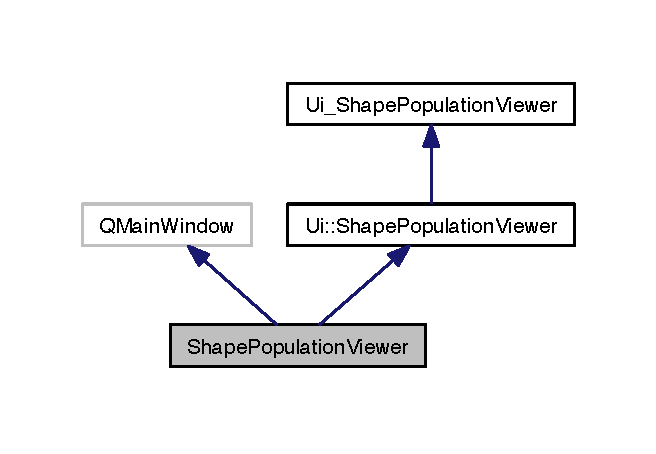
\includegraphics[width=315pt]{class_shape_population_viewer__inherit__graph}
\end{center}
\end{figure}


Collaboration diagram for Shape\-Population\-Viewer\-:\nopagebreak
\begin{figure}[H]
\begin{center}
\leavevmode
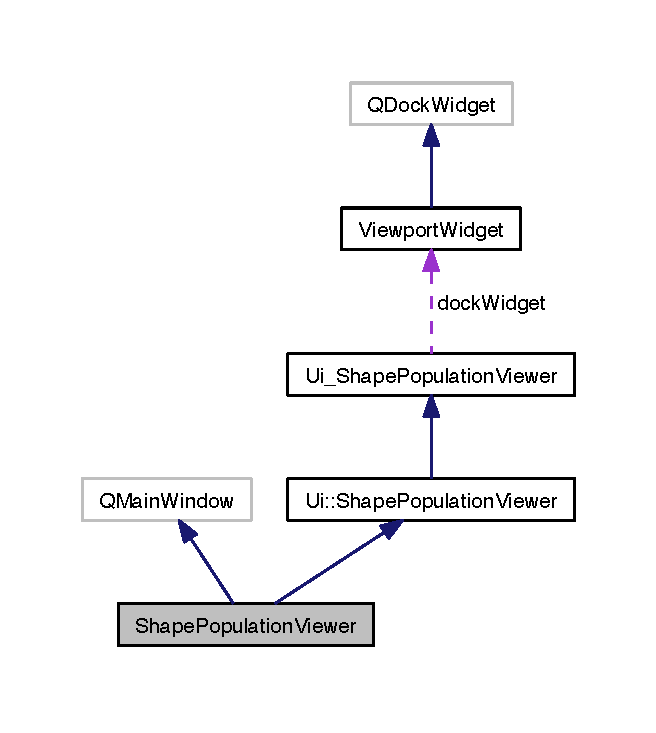
\includegraphics[width=315pt]{class_shape_population_viewer__coll__graph}
\end{center}
\end{figure}
\subsection*{Public Slots}
\begin{DoxyCompactItemize}
\item 
virtual void \hyperlink{class_shape_population_viewer_a4e328326e343af33bbb6f50368b60fe3}{slot\-Exit} ()
\begin{DoxyCompactList}\small\item\em \hyperlink{class_shape_population_viewer_a4e328326e343af33bbb6f50368b60fe3}{Shape\-Population\-Viewer\-::slot\-Exit}. \end{DoxyCompactList}\end{DoxyCompactItemize}
\subsection*{Public Member Functions}
\begin{DoxyCompactItemize}
\item 
\hyperlink{class_shape_population_viewer_a4f1a26145a1354b29b7b42a02dc8b1cf}{Shape\-Population\-Viewer} ()
\begin{DoxyCompactList}\small\item\em \hyperlink{class_shape_population_viewer_a4f1a26145a1354b29b7b42a02dc8b1cf}{Shape\-Population\-Viewer\-::\-Shape\-Population\-Viewer}. \end{DoxyCompactList}\item 
\hyperlink{class_shape_population_viewer_ae934a47a97a0a578d72ead0b94e4d9aa}{$\sim$\-Shape\-Population\-Viewer} ()
\end{DoxyCompactItemize}
\subsection*{Protected Slots}
\begin{DoxyCompactItemize}
\item 
void \hyperlink{class_shape_population_viewer_a91b876667179929c024a505a275783a6}{on\-\_\-check\-Box\-\_\-9\-\_\-toggled} (bool checked)
\begin{DoxyCompactList}\small\item\em \hyperlink{class_shape_population_viewer_a91b876667179929c024a505a275783a6}{Shape\-Population\-Viewer\-::on\-\_\-check\-Box\-\_\-9\-\_\-toggled}. \end{DoxyCompactList}\item 
void \hyperlink{class_shape_population_viewer_a272c7bf9b39d094ad66568000e8471c0}{flip\-Meshes} ()
\begin{DoxyCompactList}\small\item\em \hyperlink{class_shape_population_viewer_a272c7bf9b39d094ad66568000e8471c0}{Shape\-Population\-Viewer\-::flip\-Meshes}. \end{DoxyCompactList}\item 
void \hyperlink{class_shape_population_viewer_afa9af662d31268f494c205ab524e721c}{write\-Meshes} ()
\begin{DoxyCompactList}\small\item\em \hyperlink{class_shape_population_viewer_afa9af662d31268f494c205ab524e721c}{Shape\-Population\-Viewer\-::write\-Meshes}. \end{DoxyCompactList}\item 
void \hyperlink{class_shape_population_viewer_aa73417b59af3f879f79b42f2d2ca1e7f}{open\-V\-T\-K\-S} ()
\begin{DoxyCompactList}\small\item\em \hyperlink{class_shape_population_viewer_aa73417b59af3f879f79b42f2d2ca1e7f}{Shape\-Population\-Viewer\-::open\-V\-T\-K\-S}. \end{DoxyCompactList}\item 
void \hyperlink{class_shape_population_viewer_a962f1efd33b8d4fe3e28181a37d9aa30}{on\-\_\-check\-Box\-\_\-10\-\_\-toggled} (bool checked)
\begin{DoxyCompactList}\small\item\em \hyperlink{class_shape_population_viewer_a962f1efd33b8d4fe3e28181a37d9aa30}{Shape\-Population\-Viewer\-::on\-\_\-check\-Box\-\_\-10\-\_\-toggled}. \end{DoxyCompactList}\item 
void \hyperlink{class_shape_population_viewer_a06a4d48a520555530733a673684ba4f4}{on\-\_\-line\-Edit\-\_\-editing\-Finished} ()
\begin{DoxyCompactList}\small\item\em \hyperlink{class_shape_population_viewer_a06a4d48a520555530733a673684ba4f4}{Shape\-Population\-Viewer\-::on\-\_\-line\-Edit\-\_\-editing\-Finished}. \end{DoxyCompactList}\item 
void \hyperlink{class_shape_population_viewer_a9114bc279e8e03e21480e184c1057c8f}{on\-\_\-check\-Box\-\_\-3\-\_\-toggled} (bool checked)
\begin{DoxyCompactList}\small\item\em \hyperlink{class_shape_population_viewer_a9114bc279e8e03e21480e184c1057c8f}{Shape\-Population\-Viewer\-::on\-\_\-check\-Box\-\_\-3\-\_\-toggled}. \end{DoxyCompactList}\item 
void \hyperlink{class_shape_population_viewer_a4516673df0b16aa9b783e4b64f56fad8}{on\-\_\-combo\-Box\-\_\-current\-Index\-Changed} (const Q\-String \&arg1)
\begin{DoxyCompactList}\small\item\em \hyperlink{class_shape_population_viewer_a4516673df0b16aa9b783e4b64f56fad8}{Shape\-Population\-Viewer\-::on\-\_\-combo\-Box\-\_\-current\-Index\-Changed}. \end{DoxyCompactList}\item 
void \hyperlink{class_shape_population_viewer_afe0890a97a545e451c4b9e745fd812f0}{on\-\_\-tool\-Button\-\_\-clicked} ()
\begin{DoxyCompactList}\small\item\em \hyperlink{class_shape_population_viewer_afe0890a97a545e451c4b9e745fd812f0}{Shape\-Population\-Viewer\-::on\-\_\-tool\-Button\-\_\-clicked}. \end{DoxyCompactList}\item 
void \hyperlink{class_shape_population_viewer_a6d153b4e3b16b044581b842cdd638f4d}{on\-\_\-tool\-Button\-\_\-2\-\_\-clicked} ()
\begin{DoxyCompactList}\small\item\em \hyperlink{class_shape_population_viewer_afe0890a97a545e451c4b9e745fd812f0}{Shape\-Population\-Viewer\-::on\-\_\-tool\-Button\-\_\-clicked}. \end{DoxyCompactList}\item 
void \hyperlink{class_shape_population_viewer_a23d32bc06c2b04a34cdb504ce154c30e}{on\-\_\-tool\-Button\-\_\-3\-\_\-clicked} ()
\begin{DoxyCompactList}\small\item\em \hyperlink{class_shape_population_viewer_afe0890a97a545e451c4b9e745fd812f0}{Shape\-Population\-Viewer\-::on\-\_\-tool\-Button\-\_\-clicked}. \end{DoxyCompactList}\item 
void \hyperlink{class_shape_population_viewer_ae55f17f846f6e095898b7a78fcb8f39a}{on\-\_\-tool\-Button\-\_\-4\-\_\-clicked} ()
\begin{DoxyCompactList}\small\item\em \hyperlink{class_shape_population_viewer_afe0890a97a545e451c4b9e745fd812f0}{Shape\-Population\-Viewer\-::on\-\_\-tool\-Button\-\_\-clicked}. \end{DoxyCompactList}\item 
void \hyperlink{class_shape_population_viewer_a0282bb576425b0c916c8a08d77f02d40}{on\-\_\-tool\-Button\-\_\-5\-\_\-clicked} ()
\begin{DoxyCompactList}\small\item\em \hyperlink{class_shape_population_viewer_afe0890a97a545e451c4b9e745fd812f0}{Shape\-Population\-Viewer\-::on\-\_\-tool\-Button\-\_\-clicked}. \end{DoxyCompactList}\item 
void \hyperlink{class_shape_population_viewer_aaaef8b747a8f15bc59fb63c426111f88}{on\-\_\-tool\-Button\-\_\-6\-\_\-clicked} ()
\begin{DoxyCompactList}\small\item\em \hyperlink{class_shape_population_viewer_afe0890a97a545e451c4b9e745fd812f0}{Shape\-Population\-Viewer\-::on\-\_\-tool\-Button\-\_\-clicked}. \end{DoxyCompactList}\item 
void \hyperlink{class_shape_population_viewer_a124d5f1057623616c3e33afb50d61eeb}{view\-Change} (int x, int y, int z)
\begin{DoxyCompactList}\small\item\em \hyperlink{class_shape_population_viewer_a124d5f1057623616c3e33afb50d61eeb}{Shape\-Population\-Viewer\-::view\-Change}. \end{DoxyCompactList}\end{DoxyCompactItemize}
\subsection*{Protected Member Functions}
\begin{DoxyCompactItemize}
\item 
void \hyperlink{class_shape_population_viewer_a7b0372882e3ed9407950cce2446d2c2e}{Modified\-Handler} ()
\begin{DoxyCompactList}\small\item\em \hyperlink{class_shape_population_viewer_a7b0372882e3ed9407950cce2446d2c2e}{Shape\-Population\-Viewer\-::\-Modified\-Handler}. \end{DoxyCompactList}\item 
void \hyperlink{class_shape_population_viewer_ae4f86b69e03ff6fe171055ef3284c2ae}{resize\-Event} (Q\-Resize\-Event $\ast$event)
\begin{DoxyCompactList}\small\item\em \hyperlink{class_shape_population_viewer_ae4f86b69e03ff6fe171055ef3284c2ae}{Shape\-Population\-Viewer\-::resize\-Event}. \end{DoxyCompactList}\item 
void \hyperlink{class_shape_population_viewer_aad65b6f3730b35df25452677b6d790e1}{update\-Widgets} ()
\begin{DoxyCompactList}\small\item\em \hyperlink{class_shape_population_viewer_aad65b6f3730b35df25452677b6d790e1}{Shape\-Population\-Viewer\-::update\-Widgets}. \end{DoxyCompactList}\item 
void \hyperlink{class_shape_population_viewer_a304c6d435fab8f04099d2bc42185f74b}{update\-C\-Maps} ()
\begin{DoxyCompactList}\small\item\em \hyperlink{class_shape_population_viewer_a304c6d435fab8f04099d2bc42185f74b}{Shape\-Population\-Viewer\-::update\-C\-Maps}. \end{DoxyCompactList}\end{DoxyCompactItemize}
\subsection*{Protected Attributes}
\begin{DoxyCompactItemize}
\item 
bool \hyperlink{class_shape_population_viewer_a42b6a8e7a7b2c90615e73c80988f547d}{synced}
\item 
Q\-Dir \hyperlink{class_shape_population_viewer_aa466212a0536242cedb4233e4cf6492b}{directory}
\item 
Q\-Vector$<$ Q\-V\-T\-K\-Widget $\ast$ $>$ $\ast$ \hyperlink{class_shape_population_viewer_adaf84d2191b3d5452455bf43864ad2f2}{widget\-List}
\item 
Q\-Vector$<$ vtk\-Poly\-Data $\ast$ $>$ $\ast$ \hyperlink{class_shape_population_viewer_a5533e0d642467a70e349fa79a24bfc51}{poly\-List}
\item 
Q\-Vector$<$ vtk\-Poly\-Data\-Mapper $\ast$ $>$ $\ast$ \hyperlink{class_shape_population_viewer_a512b562448c7236c0c1bdf981a0a7322}{mapper\-List}
\item 
Q\-Vector$<$ Q\-String $>$ $\ast$ \hyperlink{class_shape_population_viewer_aefdd9f2ac19f0e0cd7bdfeb2a94dbcf3}{color\-Maps}
\item 
Q\-Size \hyperlink{class_shape_population_viewer_ae3bbe127e4bac8870cb476084a6d4917}{scroll\-Area\-Size}
\item 
Q\-String \hyperlink{class_shape_population_viewer_a69f478eade0bf23b94037e5a09dfc127}{cmap}
\item 
double $\ast$ \hyperlink{class_shape_population_viewer_aaf35bd7b070b3cef6fa85cd1f07f5ab0}{coords}
\item 
double \hyperlink{class_shape_population_viewer_a55229dfa2500b5417e5afafefcee1e0e}{distance}
\item 
int \hyperlink{class_shape_population_viewer_aa9022fa806169eef3b46a053cc1e11ce}{prev\-Cols}
\item 
int \hyperlink{class_shape_population_viewer_adb72d49a80c7536e0d7ecad1ce3b7fda}{prev\-Rows}
\item 
int \hyperlink{class_shape_population_viewer_a722158753a5d11f2f618d59ae743cb0c}{phi}
\item 
double \hyperlink{class_shape_population_viewer_a9b68299dba604343c319858e005ef644}{P\-I}
\item 
int \hyperlink{class_shape_population_viewer_a6e4ce4ade82b335f5a69ddf054314f16}{loaded}
\item 
int \hyperlink{class_shape_population_viewer_a083b364b39e12244501aca559b68708f}{sequence}
\end{DoxyCompactItemize}
\subsection*{Additional Inherited Members}


\subsection{Detailed Description}
The \hyperlink{class_shape_population_viewer}{Shape\-Population\-Viewer} class. 

\hyperlink{class_shape_population_viewer}{Shape\-Population\-Viewer} Gui class specification. This class contains all model data and controller callbacks, if we are going to consider the code within the M\-V\-C paradigm. See \hyperlink{ui___shape_population_viewer_8h}{ui\-\_\-\-Shape\-Population\-Viewer.\-h} for information on the construction of the gui itself. That is an autogenerated file from the Shape\-Population\-Viewer.\-ui file, which could also be used as reference. \begin{DoxyAuthor}{Author}
Michael Guarino 
\end{DoxyAuthor}


\subsection{Constructor \& Destructor Documentation}
\hypertarget{class_shape_population_viewer_a4f1a26145a1354b29b7b42a02dc8b1cf}{\index{Shape\-Population\-Viewer@{Shape\-Population\-Viewer}!Shape\-Population\-Viewer@{Shape\-Population\-Viewer}}
\index{Shape\-Population\-Viewer@{Shape\-Population\-Viewer}!ShapePopulationViewer@{Shape\-Population\-Viewer}}
\subsubsection[{Shape\-Population\-Viewer}]{\setlength{\rightskip}{0pt plus 5cm}Shape\-Population\-Viewer\-::\-Shape\-Population\-Viewer (
\begin{DoxyParamCaption}
{}
\end{DoxyParamCaption}
)}}\label{class_shape_population_viewer_a4f1a26145a1354b29b7b42a02dc8b1cf}


\hyperlink{class_shape_population_viewer_a4f1a26145a1354b29b7b42a02dc8b1cf}{Shape\-Population\-Viewer\-::\-Shape\-Population\-Viewer}. 

Constructor for \hyperlink{class_shape_population_viewer}{Shape\-Population\-Viewer} G\-U\-I, it will initialize model vectors, connect some callbacks and also draw the arrow icons. \begin{DoxyAuthor}{Author}
Michael Guarino 
\end{DoxyAuthor}


References Ui\-\_\-\-Shape\-Population\-Viewer\-::action\-Exit, Ui\-\_\-\-Shape\-Population\-Viewer\-::action\-Flip\-\_\-\-Meshes, Ui\-\_\-\-Shape\-Population\-Viewer\-::action\-Open\-\_\-vtk\-\_\-\-Files, Ui\-\_\-\-Shape\-Population\-Viewer\-::action\-Write\-\_\-\-Back\-\_\-\-Meshes, color\-Maps, flip\-Meshes(), loaded, mapper\-List, open\-V\-T\-K\-S(), phi, P\-I, poly\-List, Ui\-\_\-\-Shape\-Population\-Viewer\-::setup\-Ui(), slot\-Exit(), synced, Ui\-\_\-\-Shape\-Population\-Viewer\-::tool\-Button, Ui\-\_\-\-Shape\-Population\-Viewer\-::tool\-Button\-\_\-2, Ui\-\_\-\-Shape\-Population\-Viewer\-::tool\-Button\-\_\-3, Ui\-\_\-\-Shape\-Population\-Viewer\-::tool\-Button\-\_\-4, Ui\-\_\-\-Shape\-Population\-Viewer\-::tool\-Button\-\_\-5, Ui\-\_\-\-Shape\-Population\-Viewer\-::tool\-Button\-\_\-6, widget\-List, and write\-Meshes().

\hypertarget{class_shape_population_viewer_ae934a47a97a0a578d72ead0b94e4d9aa}{\index{Shape\-Population\-Viewer@{Shape\-Population\-Viewer}!$\sim$\-Shape\-Population\-Viewer@{$\sim$\-Shape\-Population\-Viewer}}
\index{$\sim$\-Shape\-Population\-Viewer@{$\sim$\-Shape\-Population\-Viewer}!ShapePopulationViewer@{Shape\-Population\-Viewer}}
\subsubsection[{$\sim$\-Shape\-Population\-Viewer}]{\setlength{\rightskip}{0pt plus 5cm}Shape\-Population\-Viewer\-::$\sim$\-Shape\-Population\-Viewer (
\begin{DoxyParamCaption}
{}
\end{DoxyParamCaption}
)\hspace{0.3cm}{\ttfamily [inline]}}}\label{class_shape_population_viewer_ae934a47a97a0a578d72ead0b94e4d9aa}


\subsection{Member Function Documentation}
\hypertarget{class_shape_population_viewer_a272c7bf9b39d094ad66568000e8471c0}{\index{Shape\-Population\-Viewer@{Shape\-Population\-Viewer}!flip\-Meshes@{flip\-Meshes}}
\index{flip\-Meshes@{flip\-Meshes}!ShapePopulationViewer@{Shape\-Population\-Viewer}}
\subsubsection[{flip\-Meshes}]{\setlength{\rightskip}{0pt plus 5cm}void Shape\-Population\-Viewer\-::flip\-Meshes (
\begin{DoxyParamCaption}
{}
\end{DoxyParamCaption}
)\hspace{0.3cm}{\ttfamily [protected]}, {\ttfamily [slot]}}}\label{class_shape_population_viewer_a272c7bf9b39d094ad66568000e8471c0}


\hyperlink{class_shape_population_viewer_a272c7bf9b39d094ad66568000e8471c0}{Shape\-Population\-Viewer\-::flip\-Meshes}. 

Callback for the flip meshes menu item, this function remaps the scalars in the specified meshes to simulate a polar shift in the parameterization. No remapping of the pointdata individuals is performed, though. \begin{DoxyAuthor}{Author}
Michael Guarino 
\end{DoxyAuthor}


References Modified\-Handler(), and poly\-List.



Referenced by Shape\-Population\-Viewer().

\hypertarget{class_shape_population_viewer_a7b0372882e3ed9407950cce2446d2c2e}{\index{Shape\-Population\-Viewer@{Shape\-Population\-Viewer}!Modified\-Handler@{Modified\-Handler}}
\index{Modified\-Handler@{Modified\-Handler}!ShapePopulationViewer@{Shape\-Population\-Viewer}}
\subsubsection[{Modified\-Handler}]{\setlength{\rightskip}{0pt plus 5cm}void Shape\-Population\-Viewer\-::\-Modified\-Handler (
\begin{DoxyParamCaption}
{}
\end{DoxyParamCaption}
)\hspace{0.3cm}{\ttfamily [protected]}}}\label{class_shape_population_viewer_a7b0372882e3ed9407950cce2446d2c2e}


\hyperlink{class_shape_population_viewer_a7b0372882e3ed9407950cce2446d2c2e}{Shape\-Population\-Viewer\-::\-Modified\-Handler}. 

Handler to any modified event sent by a Q\-V\-T\-K\-Widget in the viewport. The handler calls render on all the windows provided user is viewing in synchronized mode. \begin{DoxyAuthor}{Author}
Michael Guarino 
\end{DoxyAuthor}


References synced, and widget\-List.



Referenced by flip\-Meshes(), on\-\_\-combo\-Box\-\_\-current\-Index\-Changed(), update\-Widgets(), and view\-Change().

\hypertarget{class_shape_population_viewer_a962f1efd33b8d4fe3e28181a37d9aa30}{\index{Shape\-Population\-Viewer@{Shape\-Population\-Viewer}!on\-\_\-check\-Box\-\_\-10\-\_\-toggled@{on\-\_\-check\-Box\-\_\-10\-\_\-toggled}}
\index{on\-\_\-check\-Box\-\_\-10\-\_\-toggled@{on\-\_\-check\-Box\-\_\-10\-\_\-toggled}!ShapePopulationViewer@{Shape\-Population\-Viewer}}
\subsubsection[{on\-\_\-check\-Box\-\_\-10\-\_\-toggled}]{\setlength{\rightskip}{0pt plus 5cm}void Shape\-Population\-Viewer\-::on\-\_\-check\-Box\-\_\-10\-\_\-toggled (
\begin{DoxyParamCaption}
\item[{bool}]{checked}
\end{DoxyParamCaption}
)\hspace{0.3cm}{\ttfamily [protected]}, {\ttfamily [slot]}}}\label{class_shape_population_viewer_a962f1efd33b8d4fe3e28181a37d9aa30}


\hyperlink{class_shape_population_viewer_a962f1efd33b8d4fe3e28181a37d9aa30}{Shape\-Population\-Viewer\-::on\-\_\-check\-Box\-\_\-10\-\_\-toggled}. 

Callback for the View in \-\_\-\-\_\-\-\_\- columns checkbox. This reads from the \-\_\-\-\_\-\-\_\- columns line edit, and then re-\/arranges the Q\-V\-T\-K\-Widgets according to the integer entry. Returns if an integer is not entered (or if the same integer was reentered or if there are no widgets to rearrange). 
\begin{DoxyParams}{Parameters}
{\em checked} & \\
\hline
\end{DoxyParams}
\begin{DoxyAuthor}{Author}
Michael Guarino 
\end{DoxyAuthor}


References Ui\-\_\-\-Shape\-Population\-Viewer\-::check\-Box\-\_\-9, Ui\-\_\-\-Shape\-Population\-Viewer\-::line\-Edit, prev\-Cols, prev\-Rows, Ui\-\_\-\-Shape\-Population\-Viewer\-::scroll\-Area\-Widget\-Contents, and widget\-List.



Referenced by on\-\_\-line\-Edit\-\_\-editing\-Finished().

\hypertarget{class_shape_population_viewer_a9114bc279e8e03e21480e184c1057c8f}{\index{Shape\-Population\-Viewer@{Shape\-Population\-Viewer}!on\-\_\-check\-Box\-\_\-3\-\_\-toggled@{on\-\_\-check\-Box\-\_\-3\-\_\-toggled}}
\index{on\-\_\-check\-Box\-\_\-3\-\_\-toggled@{on\-\_\-check\-Box\-\_\-3\-\_\-toggled}!ShapePopulationViewer@{Shape\-Population\-Viewer}}
\subsubsection[{on\-\_\-check\-Box\-\_\-3\-\_\-toggled}]{\setlength{\rightskip}{0pt plus 5cm}void Shape\-Population\-Viewer\-::on\-\_\-check\-Box\-\_\-3\-\_\-toggled (
\begin{DoxyParamCaption}
\item[{bool}]{checked}
\end{DoxyParamCaption}
)\hspace{0.3cm}{\ttfamily [protected]}, {\ttfamily [slot]}}}\label{class_shape_population_viewer_a9114bc279e8e03e21480e184c1057c8f}


\hyperlink{class_shape_population_viewer_a9114bc279e8e03e21480e184c1057c8f}{Shape\-Population\-Viewer\-::on\-\_\-check\-Box\-\_\-3\-\_\-toggled}. 

Callback to the Desynchronize Meshes checkbox. Sets the synced instance variable. 
\begin{DoxyParams}{Parameters}
{\em checked} & \\
\hline
\end{DoxyParams}
\begin{DoxyAuthor}{Author}
Michael Guarino 
\end{DoxyAuthor}


References synced.

\hypertarget{class_shape_population_viewer_a91b876667179929c024a505a275783a6}{\index{Shape\-Population\-Viewer@{Shape\-Population\-Viewer}!on\-\_\-check\-Box\-\_\-9\-\_\-toggled@{on\-\_\-check\-Box\-\_\-9\-\_\-toggled}}
\index{on\-\_\-check\-Box\-\_\-9\-\_\-toggled@{on\-\_\-check\-Box\-\_\-9\-\_\-toggled}!ShapePopulationViewer@{Shape\-Population\-Viewer}}
\subsubsection[{on\-\_\-check\-Box\-\_\-9\-\_\-toggled}]{\setlength{\rightskip}{0pt plus 5cm}void Shape\-Population\-Viewer\-::on\-\_\-check\-Box\-\_\-9\-\_\-toggled (
\begin{DoxyParamCaption}
\item[{bool}]{checked}
\end{DoxyParamCaption}
)\hspace{0.3cm}{\ttfamily [protected]}, {\ttfamily [slot]}}}\label{class_shape_population_viewer_a91b876667179929c024a505a275783a6}


\hyperlink{class_shape_population_viewer_a91b876667179929c024a505a275783a6}{Shape\-Population\-Viewer\-::on\-\_\-check\-Box\-\_\-9\-\_\-toggled}. 

Callback for the View All Meshes checkbox. 
\begin{DoxyParams}{Parameters}
{\em checked} & \\
\hline
\end{DoxyParams}
\begin{DoxyAuthor}{Author}
Michael Guarino 
\end{DoxyAuthor}


References Ui\-\_\-\-Shape\-Population\-Viewer\-::check\-Box\-\_\-10, Ui\-\_\-\-Shape\-Population\-Viewer\-::scroll\-Area, scroll\-Area\-Size, and Ui\-\_\-\-Shape\-Population\-Viewer\-::scroll\-Area\-Widget\-Contents.

\hypertarget{class_shape_population_viewer_a4516673df0b16aa9b783e4b64f56fad8}{\index{Shape\-Population\-Viewer@{Shape\-Population\-Viewer}!on\-\_\-combo\-Box\-\_\-current\-Index\-Changed@{on\-\_\-combo\-Box\-\_\-current\-Index\-Changed}}
\index{on\-\_\-combo\-Box\-\_\-current\-Index\-Changed@{on\-\_\-combo\-Box\-\_\-current\-Index\-Changed}!ShapePopulationViewer@{Shape\-Population\-Viewer}}
\subsubsection[{on\-\_\-combo\-Box\-\_\-current\-Index\-Changed}]{\setlength{\rightskip}{0pt plus 5cm}void Shape\-Population\-Viewer\-::on\-\_\-combo\-Box\-\_\-current\-Index\-Changed (
\begin{DoxyParamCaption}
\item[{const Q\-String \&}]{arg1}
\end{DoxyParamCaption}
)\hspace{0.3cm}{\ttfamily [protected]}, {\ttfamily [slot]}}}\label{class_shape_population_viewer_a4516673df0b16aa9b783e4b64f56fad8}


\hyperlink{class_shape_population_viewer_a4516673df0b16aa9b783e4b64f56fad8}{Shape\-Population\-Viewer\-::on\-\_\-combo\-Box\-\_\-current\-Index\-Changed}. 

Callback to the colormap dropdown menu. This will pull the selected text from the menu, call the \hyperlink{class_shape_population_viewer_a304c6d435fab8f04099d2bc42185f74b}{update\-C\-Maps()} helper, then call Render on all the Q\-V\-T\-K\-Widgets to render the updates. 
\begin{DoxyParams}{Parameters}
{\em arg1} & \\
\hline
\end{DoxyParams}
\begin{DoxyAuthor}{Author}
Michael Guarino 
\end{DoxyAuthor}


References cmap, Ui\-\_\-\-Shape\-Population\-Viewer\-::combo\-Box, Modified\-Handler(), synced, and update\-C\-Maps().

\hypertarget{class_shape_population_viewer_a06a4d48a520555530733a673684ba4f4}{\index{Shape\-Population\-Viewer@{Shape\-Population\-Viewer}!on\-\_\-line\-Edit\-\_\-editing\-Finished@{on\-\_\-line\-Edit\-\_\-editing\-Finished}}
\index{on\-\_\-line\-Edit\-\_\-editing\-Finished@{on\-\_\-line\-Edit\-\_\-editing\-Finished}!ShapePopulationViewer@{Shape\-Population\-Viewer}}
\subsubsection[{on\-\_\-line\-Edit\-\_\-editing\-Finished}]{\setlength{\rightskip}{0pt plus 5cm}void Shape\-Population\-Viewer\-::on\-\_\-line\-Edit\-\_\-editing\-Finished (
\begin{DoxyParamCaption}
{}
\end{DoxyParamCaption}
)\hspace{0.3cm}{\ttfamily [protected]}, {\ttfamily [slot]}}}\label{class_shape_population_viewer_a06a4d48a520555530733a673684ba4f4}


\hyperlink{class_shape_population_viewer_a06a4d48a520555530733a673684ba4f4}{Shape\-Population\-Viewer\-::on\-\_\-line\-Edit\-\_\-editing\-Finished}. 

Callback to the \-\_\-\-\_\-\-\_\- columns line edit. This checks if the view in \-\_\-\-\_\-\-\_\- columns checkbox is selected, then it will simply call its callback with true passed as the check state. So a lineedit modification also activates column rearrangement. \begin{DoxyAuthor}{Author}
Michael Guarino 
\end{DoxyAuthor}


References Ui\-\_\-\-Shape\-Population\-Viewer\-::check\-Box\-\_\-10, and on\-\_\-check\-Box\-\_\-10\-\_\-toggled().

\hypertarget{class_shape_population_viewer_a6d153b4e3b16b044581b842cdd638f4d}{\index{Shape\-Population\-Viewer@{Shape\-Population\-Viewer}!on\-\_\-tool\-Button\-\_\-2\-\_\-clicked@{on\-\_\-tool\-Button\-\_\-2\-\_\-clicked}}
\index{on\-\_\-tool\-Button\-\_\-2\-\_\-clicked@{on\-\_\-tool\-Button\-\_\-2\-\_\-clicked}!ShapePopulationViewer@{Shape\-Population\-Viewer}}
\subsubsection[{on\-\_\-tool\-Button\-\_\-2\-\_\-clicked}]{\setlength{\rightskip}{0pt plus 5cm}void Shape\-Population\-Viewer\-::on\-\_\-tool\-Button\-\_\-2\-\_\-clicked (
\begin{DoxyParamCaption}
{}
\end{DoxyParamCaption}
)\hspace{0.3cm}{\ttfamily [protected]}, {\ttfamily [slot]}}}\label{class_shape_population_viewer_a6d153b4e3b16b044581b842cdd638f4d}


\hyperlink{class_shape_population_viewer_afe0890a97a545e451c4b9e745fd812f0}{Shape\-Population\-Viewer\-::on\-\_\-tool\-Button\-\_\-clicked}. 

Callback to the -\/\-Z axis view button. See \hyperlink{class_shape_population_viewer_a124d5f1057623616c3e33afb50d61eeb}{view\-Change()} for implemntation details. \begin{DoxyAuthor}{Author}
Joe Waggoner 
\end{DoxyAuthor}


References view\-Change().

\hypertarget{class_shape_population_viewer_a23d32bc06c2b04a34cdb504ce154c30e}{\index{Shape\-Population\-Viewer@{Shape\-Population\-Viewer}!on\-\_\-tool\-Button\-\_\-3\-\_\-clicked@{on\-\_\-tool\-Button\-\_\-3\-\_\-clicked}}
\index{on\-\_\-tool\-Button\-\_\-3\-\_\-clicked@{on\-\_\-tool\-Button\-\_\-3\-\_\-clicked}!ShapePopulationViewer@{Shape\-Population\-Viewer}}
\subsubsection[{on\-\_\-tool\-Button\-\_\-3\-\_\-clicked}]{\setlength{\rightskip}{0pt plus 5cm}void Shape\-Population\-Viewer\-::on\-\_\-tool\-Button\-\_\-3\-\_\-clicked (
\begin{DoxyParamCaption}
{}
\end{DoxyParamCaption}
)\hspace{0.3cm}{\ttfamily [protected]}, {\ttfamily [slot]}}}\label{class_shape_population_viewer_a23d32bc06c2b04a34cdb504ce154c30e}


\hyperlink{class_shape_population_viewer_afe0890a97a545e451c4b9e745fd812f0}{Shape\-Population\-Viewer\-::on\-\_\-tool\-Button\-\_\-clicked}. 

Callback to the +\-X axis view button. See \hyperlink{class_shape_population_viewer_a124d5f1057623616c3e33afb50d61eeb}{view\-Change()} for implemntation details. \begin{DoxyAuthor}{Author}
Joe Waggoner 
\end{DoxyAuthor}


References view\-Change().

\hypertarget{class_shape_population_viewer_ae55f17f846f6e095898b7a78fcb8f39a}{\index{Shape\-Population\-Viewer@{Shape\-Population\-Viewer}!on\-\_\-tool\-Button\-\_\-4\-\_\-clicked@{on\-\_\-tool\-Button\-\_\-4\-\_\-clicked}}
\index{on\-\_\-tool\-Button\-\_\-4\-\_\-clicked@{on\-\_\-tool\-Button\-\_\-4\-\_\-clicked}!ShapePopulationViewer@{Shape\-Population\-Viewer}}
\subsubsection[{on\-\_\-tool\-Button\-\_\-4\-\_\-clicked}]{\setlength{\rightskip}{0pt plus 5cm}void Shape\-Population\-Viewer\-::on\-\_\-tool\-Button\-\_\-4\-\_\-clicked (
\begin{DoxyParamCaption}
{}
\end{DoxyParamCaption}
)\hspace{0.3cm}{\ttfamily [protected]}, {\ttfamily [slot]}}}\label{class_shape_population_viewer_ae55f17f846f6e095898b7a78fcb8f39a}


\hyperlink{class_shape_population_viewer_afe0890a97a545e451c4b9e745fd812f0}{Shape\-Population\-Viewer\-::on\-\_\-tool\-Button\-\_\-clicked}. 

Callback to the -\/\-X axis view button. See \hyperlink{class_shape_population_viewer_a124d5f1057623616c3e33afb50d61eeb}{view\-Change()} for implemntation details. \begin{DoxyAuthor}{Author}
Joe Waggoner 
\end{DoxyAuthor}


References view\-Change().

\hypertarget{class_shape_population_viewer_a0282bb576425b0c916c8a08d77f02d40}{\index{Shape\-Population\-Viewer@{Shape\-Population\-Viewer}!on\-\_\-tool\-Button\-\_\-5\-\_\-clicked@{on\-\_\-tool\-Button\-\_\-5\-\_\-clicked}}
\index{on\-\_\-tool\-Button\-\_\-5\-\_\-clicked@{on\-\_\-tool\-Button\-\_\-5\-\_\-clicked}!ShapePopulationViewer@{Shape\-Population\-Viewer}}
\subsubsection[{on\-\_\-tool\-Button\-\_\-5\-\_\-clicked}]{\setlength{\rightskip}{0pt plus 5cm}void Shape\-Population\-Viewer\-::on\-\_\-tool\-Button\-\_\-5\-\_\-clicked (
\begin{DoxyParamCaption}
{}
\end{DoxyParamCaption}
)\hspace{0.3cm}{\ttfamily [protected]}, {\ttfamily [slot]}}}\label{class_shape_population_viewer_a0282bb576425b0c916c8a08d77f02d40}


\hyperlink{class_shape_population_viewer_afe0890a97a545e451c4b9e745fd812f0}{Shape\-Population\-Viewer\-::on\-\_\-tool\-Button\-\_\-clicked}. 

Callback to the +\-Y axis view button. See \hyperlink{class_shape_population_viewer_a124d5f1057623616c3e33afb50d61eeb}{view\-Change()} for implemntation details. \begin{DoxyAuthor}{Author}
Joe Waggoner 
\end{DoxyAuthor}


References view\-Change().

\hypertarget{class_shape_population_viewer_aaaef8b747a8f15bc59fb63c426111f88}{\index{Shape\-Population\-Viewer@{Shape\-Population\-Viewer}!on\-\_\-tool\-Button\-\_\-6\-\_\-clicked@{on\-\_\-tool\-Button\-\_\-6\-\_\-clicked}}
\index{on\-\_\-tool\-Button\-\_\-6\-\_\-clicked@{on\-\_\-tool\-Button\-\_\-6\-\_\-clicked}!ShapePopulationViewer@{Shape\-Population\-Viewer}}
\subsubsection[{on\-\_\-tool\-Button\-\_\-6\-\_\-clicked}]{\setlength{\rightskip}{0pt plus 5cm}void Shape\-Population\-Viewer\-::on\-\_\-tool\-Button\-\_\-6\-\_\-clicked (
\begin{DoxyParamCaption}
{}
\end{DoxyParamCaption}
)\hspace{0.3cm}{\ttfamily [protected]}, {\ttfamily [slot]}}}\label{class_shape_population_viewer_aaaef8b747a8f15bc59fb63c426111f88}


\hyperlink{class_shape_population_viewer_afe0890a97a545e451c4b9e745fd812f0}{Shape\-Population\-Viewer\-::on\-\_\-tool\-Button\-\_\-clicked}. 

Callback to the -\/\-Y axis view button. See \hyperlink{class_shape_population_viewer_a124d5f1057623616c3e33afb50d61eeb}{view\-Change()} for implemntation details. \begin{DoxyAuthor}{Author}
Joe Waggoner 
\end{DoxyAuthor}


References view\-Change().

\hypertarget{class_shape_population_viewer_afe0890a97a545e451c4b9e745fd812f0}{\index{Shape\-Population\-Viewer@{Shape\-Population\-Viewer}!on\-\_\-tool\-Button\-\_\-clicked@{on\-\_\-tool\-Button\-\_\-clicked}}
\index{on\-\_\-tool\-Button\-\_\-clicked@{on\-\_\-tool\-Button\-\_\-clicked}!ShapePopulationViewer@{Shape\-Population\-Viewer}}
\subsubsection[{on\-\_\-tool\-Button\-\_\-clicked}]{\setlength{\rightskip}{0pt plus 5cm}void Shape\-Population\-Viewer\-::on\-\_\-tool\-Button\-\_\-clicked (
\begin{DoxyParamCaption}
{}
\end{DoxyParamCaption}
)\hspace{0.3cm}{\ttfamily [protected]}, {\ttfamily [slot]}}}\label{class_shape_population_viewer_afe0890a97a545e451c4b9e745fd812f0}


\hyperlink{class_shape_population_viewer_afe0890a97a545e451c4b9e745fd812f0}{Shape\-Population\-Viewer\-::on\-\_\-tool\-Button\-\_\-clicked}. 

Callback to the +\-Z axis view button. See \hyperlink{class_shape_population_viewer_a124d5f1057623616c3e33afb50d61eeb}{view\-Change()} for implemntation details. \begin{DoxyAuthor}{Author}
Joe Waggoner 
\end{DoxyAuthor}


References view\-Change().

\hypertarget{class_shape_population_viewer_aa73417b59af3f879f79b42f2d2ca1e7f}{\index{Shape\-Population\-Viewer@{Shape\-Population\-Viewer}!open\-V\-T\-K\-S@{open\-V\-T\-K\-S}}
\index{open\-V\-T\-K\-S@{open\-V\-T\-K\-S}!ShapePopulationViewer@{Shape\-Population\-Viewer}}
\subsubsection[{open\-V\-T\-K\-S}]{\setlength{\rightskip}{0pt plus 5cm}void Shape\-Population\-Viewer\-::open\-V\-T\-K\-S (
\begin{DoxyParamCaption}
{}
\end{DoxyParamCaption}
)\hspace{0.3cm}{\ttfamily [protected]}, {\ttfamily [slot]}}}\label{class_shape_population_viewer_aa73417b59af3f879f79b42f2d2ca1e7f}


\hyperlink{class_shape_population_viewer_aa73417b59af3f879f79b42f2d2ca1e7f}{Shape\-Population\-Viewer\-::open\-V\-T\-K\-S}. 

Callback to Open .vtk Files menu item, this simply clears all current widgets, pulls open a filedialog to let the user select a directory and then calls the \hyperlink{class_shape_population_viewer_aad65b6f3730b35df25452677b6d790e1}{update\-Widgets()} helper function \begin{DoxyAuthor}{Author}
Michael Guarino 
\end{DoxyAuthor}


References directory, loaded, Ui\-\_\-\-Shape\-Population\-Viewer\-::scroll\-Area\-Widget\-Contents, update\-Widgets(), and widget\-List.



Referenced by Shape\-Population\-Viewer().

\hypertarget{class_shape_population_viewer_ae4f86b69e03ff6fe171055ef3284c2ae}{\index{Shape\-Population\-Viewer@{Shape\-Population\-Viewer}!resize\-Event@{resize\-Event}}
\index{resize\-Event@{resize\-Event}!ShapePopulationViewer@{Shape\-Population\-Viewer}}
\subsubsection[{resize\-Event}]{\setlength{\rightskip}{0pt plus 5cm}void Shape\-Population\-Viewer\-::resize\-Event (
\begin{DoxyParamCaption}
\item[{Q\-Resize\-Event $\ast$}]{event}
\end{DoxyParamCaption}
)\hspace{0.3cm}{\ttfamily [protected]}}}\label{class_shape_population_viewer_ae4f86b69e03ff6fe171055ef3284c2ae}


\hyperlink{class_shape_population_viewer_ae4f86b69e03ff6fe171055ef3284c2ae}{Shape\-Population\-Viewer\-::resize\-Event}. 

Overrides Q\-Main\-Window's resize event to also help resize the contents of the dockwidget's scrollarea. There is no other easy way to do this with the Qt tools as they are currently. 
\begin{DoxyParams}{Parameters}
{\em event} & -\/ variable containing the event data for a resize (needed for a super call) \\
\hline
\end{DoxyParams}
\begin{DoxyAuthor}{Author}
Michael Guarino 
\end{DoxyAuthor}


References Ui\-\_\-\-Shape\-Population\-Viewer\-::dock\-Widget, Ui\-\_\-\-Shape\-Population\-Viewer\-::scroll\-Area, Ui\-\_\-\-Shape\-Population\-Viewer\-::scroll\-Area\-Widget\-Contents, and Viewport\-Widget\-::size().

\hypertarget{class_shape_population_viewer_a4e328326e343af33bbb6f50368b60fe3}{\index{Shape\-Population\-Viewer@{Shape\-Population\-Viewer}!slot\-Exit@{slot\-Exit}}
\index{slot\-Exit@{slot\-Exit}!ShapePopulationViewer@{Shape\-Population\-Viewer}}
\subsubsection[{slot\-Exit}]{\setlength{\rightskip}{0pt plus 5cm}void Shape\-Population\-Viewer\-::slot\-Exit (
\begin{DoxyParamCaption}
{}
\end{DoxyParamCaption}
)\hspace{0.3cm}{\ttfamily [virtual]}, {\ttfamily [slot]}}}\label{class_shape_population_viewer_a4e328326e343af33bbb6f50368b60fe3}


\hyperlink{class_shape_population_viewer_a4e328326e343af33bbb6f50368b60fe3}{Shape\-Population\-Viewer\-::slot\-Exit}. 

Close function for the gui. 

Referenced by Shape\-Population\-Viewer().

\hypertarget{class_shape_population_viewer_a304c6d435fab8f04099d2bc42185f74b}{\index{Shape\-Population\-Viewer@{Shape\-Population\-Viewer}!update\-C\-Maps@{update\-C\-Maps}}
\index{update\-C\-Maps@{update\-C\-Maps}!ShapePopulationViewer@{Shape\-Population\-Viewer}}
\subsubsection[{update\-C\-Maps}]{\setlength{\rightskip}{0pt plus 5cm}void Shape\-Population\-Viewer\-::update\-C\-Maps (
\begin{DoxyParamCaption}
{}
\end{DoxyParamCaption}
)\hspace{0.3cm}{\ttfamily [protected]}}}\label{class_shape_population_viewer_a304c6d435fab8f04099d2bc42185f74b}


\hyperlink{class_shape_population_viewer_a304c6d435fab8f04099d2bc42185f74b}{Shape\-Population\-Viewer\-::update\-C\-Maps}. 

Helper function which sets the working color map to the one saved in the cmap Q\-String instance variable \begin{DoxyAuthor}{Author}
Michael Guarino 
\end{DoxyAuthor}


References cmap, mapper\-List, phi, and poly\-List.



Referenced by on\-\_\-combo\-Box\-\_\-current\-Index\-Changed().

\hypertarget{class_shape_population_viewer_aad65b6f3730b35df25452677b6d790e1}{\index{Shape\-Population\-Viewer@{Shape\-Population\-Viewer}!update\-Widgets@{update\-Widgets}}
\index{update\-Widgets@{update\-Widgets}!ShapePopulationViewer@{Shape\-Population\-Viewer}}
\subsubsection[{update\-Widgets}]{\setlength{\rightskip}{0pt plus 5cm}void Shape\-Population\-Viewer\-::update\-Widgets (
\begin{DoxyParamCaption}
{}
\end{DoxyParamCaption}
)\hspace{0.3cm}{\ttfamily [protected]}}}\label{class_shape_population_viewer_aad65b6f3730b35df25452677b6d790e1}


\hyperlink{class_shape_population_viewer_aad65b6f3730b35df25452677b6d790e1}{Shape\-Population\-Viewer\-::update\-Widgets}. 

Helper function which reads a directory filled with .vtk files and renders each polydata within in a separate Q\-V\-T\-K\-Widget. All model vectors are filled as well. \begin{DoxyAuthor}{Author}
Michael Guarino 
\end{DoxyAuthor}


References color\-Maps, Ui\-\_\-\-Shape\-Population\-Viewer\-::combo\-Box, directory, Ui\-\_\-\-Shape\-Population\-Viewer\-::line\-Edit, mapper\-List, Modified\-Handler(), phi, poly\-List, prev\-Cols, prev\-Rows, Ui\-\_\-\-Shape\-Population\-Viewer\-::scroll\-Area\-Widget\-Contents, and widget\-List.



Referenced by open\-V\-T\-K\-S().

\hypertarget{class_shape_population_viewer_a124d5f1057623616c3e33afb50d61eeb}{\index{Shape\-Population\-Viewer@{Shape\-Population\-Viewer}!view\-Change@{view\-Change}}
\index{view\-Change@{view\-Change}!ShapePopulationViewer@{Shape\-Population\-Viewer}}
\subsubsection[{view\-Change}]{\setlength{\rightskip}{0pt plus 5cm}void Shape\-Population\-Viewer\-::view\-Change (
\begin{DoxyParamCaption}
\item[{int}]{x, }
\item[{int}]{y, }
\item[{int}]{z}
\end{DoxyParamCaption}
)\hspace{0.3cm}{\ttfamily [protected]}, {\ttfamily [slot]}}}\label{class_shape_population_viewer_a124d5f1057623616c3e33afb50d61eeb}


\hyperlink{class_shape_population_viewer_a124d5f1057623616c3e33afb50d61eeb}{Shape\-Population\-Viewer\-::view\-Change}. 

Helper function for viewing the meshes along a specified axis. Parameters (1,0,0) will allow you to view the mesh from the end of the positive x-\/axis, for instance. Generally, $<$x,y,z$>$ is a distance-\/normalized vector specifying the position you want to place the viewing camera (distance being the current distance from the camera to the mesh). 
\begin{DoxyParams}{Parameters}
{\em x} & \\
\hline
{\em y} & \\
\hline
{\em z} & \\
\hline
\end{DoxyParams}
\begin{DoxyAuthor}{Author}
Joe Waggoner 
\end{DoxyAuthor}


References coords, distance, loaded, Modified\-Handler(), synced, and widget\-List.



Referenced by on\-\_\-tool\-Button\-\_\-2\-\_\-clicked(), on\-\_\-tool\-Button\-\_\-3\-\_\-clicked(), on\-\_\-tool\-Button\-\_\-4\-\_\-clicked(), on\-\_\-tool\-Button\-\_\-5\-\_\-clicked(), on\-\_\-tool\-Button\-\_\-6\-\_\-clicked(), and on\-\_\-tool\-Button\-\_\-clicked().

\hypertarget{class_shape_population_viewer_afa9af662d31268f494c205ab524e721c}{\index{Shape\-Population\-Viewer@{Shape\-Population\-Viewer}!write\-Meshes@{write\-Meshes}}
\index{write\-Meshes@{write\-Meshes}!ShapePopulationViewer@{Shape\-Population\-Viewer}}
\subsubsection[{write\-Meshes}]{\setlength{\rightskip}{0pt plus 5cm}void Shape\-Population\-Viewer\-::write\-Meshes (
\begin{DoxyParamCaption}
{}
\end{DoxyParamCaption}
)\hspace{0.3cm}{\ttfamily [protected]}, {\ttfamily [slot]}}}\label{class_shape_population_viewer_afa9af662d31268f494c205ab524e721c}


\hyperlink{class_shape_population_viewer_afa9af662d31268f494c205ab524e721c}{Shape\-Population\-Viewer\-::write\-Meshes}. 

Callback to the Write Meshes menu item, this will write every current polydata back to their original files. The choice of saving each file individually with a user specified file name was eliminated as it is entirely possible that very large numbers of meshes are going to be visualized, make that procedure tedious. \begin{DoxyAuthor}{Author}
Michael Guarino 
\end{DoxyAuthor}


References directory, and poly\-List.



Referenced by Shape\-Population\-Viewer().



\subsection{Member Data Documentation}
\hypertarget{class_shape_population_viewer_a69f478eade0bf23b94037e5a09dfc127}{\index{Shape\-Population\-Viewer@{Shape\-Population\-Viewer}!cmap@{cmap}}
\index{cmap@{cmap}!ShapePopulationViewer@{Shape\-Population\-Viewer}}
\subsubsection[{cmap}]{\setlength{\rightskip}{0pt plus 5cm}Q\-String Shape\-Population\-Viewer\-::cmap\hspace{0.3cm}{\ttfamily [protected]}}}\label{class_shape_population_viewer_a69f478eade0bf23b94037e5a09dfc127}


Referenced by on\-\_\-combo\-Box\-\_\-current\-Index\-Changed(), and update\-C\-Maps().

\hypertarget{class_shape_population_viewer_aefdd9f2ac19f0e0cd7bdfeb2a94dbcf3}{\index{Shape\-Population\-Viewer@{Shape\-Population\-Viewer}!color\-Maps@{color\-Maps}}
\index{color\-Maps@{color\-Maps}!ShapePopulationViewer@{Shape\-Population\-Viewer}}
\subsubsection[{color\-Maps}]{\setlength{\rightskip}{0pt plus 5cm}Q\-Vector$<$Q\-String$>$$\ast$ Shape\-Population\-Viewer\-::color\-Maps\hspace{0.3cm}{\ttfamily [protected]}}}\label{class_shape_population_viewer_aefdd9f2ac19f0e0cd7bdfeb2a94dbcf3}


Referenced by Shape\-Population\-Viewer(), and update\-Widgets().

\hypertarget{class_shape_population_viewer_aaf35bd7b070b3cef6fa85cd1f07f5ab0}{\index{Shape\-Population\-Viewer@{Shape\-Population\-Viewer}!coords@{coords}}
\index{coords@{coords}!ShapePopulationViewer@{Shape\-Population\-Viewer}}
\subsubsection[{coords}]{\setlength{\rightskip}{0pt plus 5cm}double$\ast$ Shape\-Population\-Viewer\-::coords\hspace{0.3cm}{\ttfamily [protected]}}}\label{class_shape_population_viewer_aaf35bd7b070b3cef6fa85cd1f07f5ab0}


Referenced by view\-Change().

\hypertarget{class_shape_population_viewer_aa466212a0536242cedb4233e4cf6492b}{\index{Shape\-Population\-Viewer@{Shape\-Population\-Viewer}!directory@{directory}}
\index{directory@{directory}!ShapePopulationViewer@{Shape\-Population\-Viewer}}
\subsubsection[{directory}]{\setlength{\rightskip}{0pt plus 5cm}Q\-Dir Shape\-Population\-Viewer\-::directory\hspace{0.3cm}{\ttfamily [protected]}}}\label{class_shape_population_viewer_aa466212a0536242cedb4233e4cf6492b}


Referenced by open\-V\-T\-K\-S(), update\-Widgets(), and write\-Meshes().

\hypertarget{class_shape_population_viewer_a55229dfa2500b5417e5afafefcee1e0e}{\index{Shape\-Population\-Viewer@{Shape\-Population\-Viewer}!distance@{distance}}
\index{distance@{distance}!ShapePopulationViewer@{Shape\-Population\-Viewer}}
\subsubsection[{distance}]{\setlength{\rightskip}{0pt plus 5cm}double Shape\-Population\-Viewer\-::distance\hspace{0.3cm}{\ttfamily [protected]}}}\label{class_shape_population_viewer_a55229dfa2500b5417e5afafefcee1e0e}


Referenced by view\-Change().

\hypertarget{class_shape_population_viewer_a6e4ce4ade82b335f5a69ddf054314f16}{\index{Shape\-Population\-Viewer@{Shape\-Population\-Viewer}!loaded@{loaded}}
\index{loaded@{loaded}!ShapePopulationViewer@{Shape\-Population\-Viewer}}
\subsubsection[{loaded}]{\setlength{\rightskip}{0pt plus 5cm}int Shape\-Population\-Viewer\-::loaded\hspace{0.3cm}{\ttfamily [protected]}}}\label{class_shape_population_viewer_a6e4ce4ade82b335f5a69ddf054314f16}


Referenced by open\-V\-T\-K\-S(), Shape\-Population\-Viewer(), and view\-Change().

\hypertarget{class_shape_population_viewer_a512b562448c7236c0c1bdf981a0a7322}{\index{Shape\-Population\-Viewer@{Shape\-Population\-Viewer}!mapper\-List@{mapper\-List}}
\index{mapper\-List@{mapper\-List}!ShapePopulationViewer@{Shape\-Population\-Viewer}}
\subsubsection[{mapper\-List}]{\setlength{\rightskip}{0pt plus 5cm}Q\-Vector$<$vtk\-Poly\-Data\-Mapper $\ast$$>$$\ast$ Shape\-Population\-Viewer\-::mapper\-List\hspace{0.3cm}{\ttfamily [protected]}}}\label{class_shape_population_viewer_a512b562448c7236c0c1bdf981a0a7322}


Referenced by Shape\-Population\-Viewer(), update\-C\-Maps(), and update\-Widgets().

\hypertarget{class_shape_population_viewer_a722158753a5d11f2f618d59ae743cb0c}{\index{Shape\-Population\-Viewer@{Shape\-Population\-Viewer}!phi@{phi}}
\index{phi@{phi}!ShapePopulationViewer@{Shape\-Population\-Viewer}}
\subsubsection[{phi}]{\setlength{\rightskip}{0pt plus 5cm}int Shape\-Population\-Viewer\-::phi\hspace{0.3cm}{\ttfamily [protected]}}}\label{class_shape_population_viewer_a722158753a5d11f2f618d59ae743cb0c}


Referenced by Shape\-Population\-Viewer(), update\-C\-Maps(), and update\-Widgets().

\hypertarget{class_shape_population_viewer_a9b68299dba604343c319858e005ef644}{\index{Shape\-Population\-Viewer@{Shape\-Population\-Viewer}!P\-I@{P\-I}}
\index{P\-I@{P\-I}!ShapePopulationViewer@{Shape\-Population\-Viewer}}
\subsubsection[{P\-I}]{\setlength{\rightskip}{0pt plus 5cm}double Shape\-Population\-Viewer\-::\-P\-I\hspace{0.3cm}{\ttfamily [protected]}}}\label{class_shape_population_viewer_a9b68299dba604343c319858e005ef644}


Referenced by Shape\-Population\-Viewer().

\hypertarget{class_shape_population_viewer_a5533e0d642467a70e349fa79a24bfc51}{\index{Shape\-Population\-Viewer@{Shape\-Population\-Viewer}!poly\-List@{poly\-List}}
\index{poly\-List@{poly\-List}!ShapePopulationViewer@{Shape\-Population\-Viewer}}
\subsubsection[{poly\-List}]{\setlength{\rightskip}{0pt plus 5cm}Q\-Vector$<$vtk\-Poly\-Data $\ast$$>$$\ast$ Shape\-Population\-Viewer\-::poly\-List\hspace{0.3cm}{\ttfamily [protected]}}}\label{class_shape_population_viewer_a5533e0d642467a70e349fa79a24bfc51}


Referenced by flip\-Meshes(), Shape\-Population\-Viewer(), update\-C\-Maps(), update\-Widgets(), and write\-Meshes().

\hypertarget{class_shape_population_viewer_aa9022fa806169eef3b46a053cc1e11ce}{\index{Shape\-Population\-Viewer@{Shape\-Population\-Viewer}!prev\-Cols@{prev\-Cols}}
\index{prev\-Cols@{prev\-Cols}!ShapePopulationViewer@{Shape\-Population\-Viewer}}
\subsubsection[{prev\-Cols}]{\setlength{\rightskip}{0pt plus 5cm}int Shape\-Population\-Viewer\-::prev\-Cols\hspace{0.3cm}{\ttfamily [protected]}}}\label{class_shape_population_viewer_aa9022fa806169eef3b46a053cc1e11ce}


Referenced by on\-\_\-check\-Box\-\_\-10\-\_\-toggled(), and update\-Widgets().

\hypertarget{class_shape_population_viewer_adb72d49a80c7536e0d7ecad1ce3b7fda}{\index{Shape\-Population\-Viewer@{Shape\-Population\-Viewer}!prev\-Rows@{prev\-Rows}}
\index{prev\-Rows@{prev\-Rows}!ShapePopulationViewer@{Shape\-Population\-Viewer}}
\subsubsection[{prev\-Rows}]{\setlength{\rightskip}{0pt plus 5cm}int Shape\-Population\-Viewer\-::prev\-Rows\hspace{0.3cm}{\ttfamily [protected]}}}\label{class_shape_population_viewer_adb72d49a80c7536e0d7ecad1ce3b7fda}


Referenced by on\-\_\-check\-Box\-\_\-10\-\_\-toggled(), and update\-Widgets().

\hypertarget{class_shape_population_viewer_ae3bbe127e4bac8870cb476084a6d4917}{\index{Shape\-Population\-Viewer@{Shape\-Population\-Viewer}!scroll\-Area\-Size@{scroll\-Area\-Size}}
\index{scroll\-Area\-Size@{scroll\-Area\-Size}!ShapePopulationViewer@{Shape\-Population\-Viewer}}
\subsubsection[{scroll\-Area\-Size}]{\setlength{\rightskip}{0pt plus 5cm}Q\-Size Shape\-Population\-Viewer\-::scroll\-Area\-Size\hspace{0.3cm}{\ttfamily [protected]}}}\label{class_shape_population_viewer_ae3bbe127e4bac8870cb476084a6d4917}


Referenced by on\-\_\-check\-Box\-\_\-9\-\_\-toggled().

\hypertarget{class_shape_population_viewer_a083b364b39e12244501aca559b68708f}{\index{Shape\-Population\-Viewer@{Shape\-Population\-Viewer}!sequence@{sequence}}
\index{sequence@{sequence}!ShapePopulationViewer@{Shape\-Population\-Viewer}}
\subsubsection[{sequence}]{\setlength{\rightskip}{0pt plus 5cm}int Shape\-Population\-Viewer\-::sequence\hspace{0.3cm}{\ttfamily [protected]}}}\label{class_shape_population_viewer_a083b364b39e12244501aca559b68708f}
\hypertarget{class_shape_population_viewer_a42b6a8e7a7b2c90615e73c80988f547d}{\index{Shape\-Population\-Viewer@{Shape\-Population\-Viewer}!synced@{synced}}
\index{synced@{synced}!ShapePopulationViewer@{Shape\-Population\-Viewer}}
\subsubsection[{synced}]{\setlength{\rightskip}{0pt plus 5cm}bool Shape\-Population\-Viewer\-::synced\hspace{0.3cm}{\ttfamily [protected]}}}\label{class_shape_population_viewer_a42b6a8e7a7b2c90615e73c80988f547d}


Referenced by Modified\-Handler(), on\-\_\-check\-Box\-\_\-3\-\_\-toggled(), on\-\_\-combo\-Box\-\_\-current\-Index\-Changed(), Shape\-Population\-Viewer(), and view\-Change().

\hypertarget{class_shape_population_viewer_adaf84d2191b3d5452455bf43864ad2f2}{\index{Shape\-Population\-Viewer@{Shape\-Population\-Viewer}!widget\-List@{widget\-List}}
\index{widget\-List@{widget\-List}!ShapePopulationViewer@{Shape\-Population\-Viewer}}
\subsubsection[{widget\-List}]{\setlength{\rightskip}{0pt plus 5cm}Q\-Vector$<$Q\-V\-T\-K\-Widget $\ast$$>$$\ast$ Shape\-Population\-Viewer\-::widget\-List\hspace{0.3cm}{\ttfamily [protected]}}}\label{class_shape_population_viewer_adaf84d2191b3d5452455bf43864ad2f2}


Referenced by Modified\-Handler(), on\-\_\-check\-Box\-\_\-10\-\_\-toggled(), open\-V\-T\-K\-S(), Shape\-Population\-Viewer(), update\-Widgets(), and view\-Change().



The documentation for this class was generated from the following files\-:\begin{DoxyCompactItemize}
\item 
\hyperlink{_shape_population_viewer_8h}{Shape\-Population\-Viewer.\-h}\item 
\hyperlink{_shape_population_viewer_8cxx}{Shape\-Population\-Viewer.\-cxx}\end{DoxyCompactItemize}

\hypertarget{class_ui_1_1_shape_population_viewer}{\section{Ui\-:\-:Shape\-Population\-Viewer Class Reference}
\label{class_ui_1_1_shape_population_viewer}\index{Ui\-::\-Shape\-Population\-Viewer@{Ui\-::\-Shape\-Population\-Viewer}}
}


Inheritance diagram for Ui\-:\-:Shape\-Population\-Viewer\-:\nopagebreak
\begin{figure}[H]
\begin{center}
\leavevmode
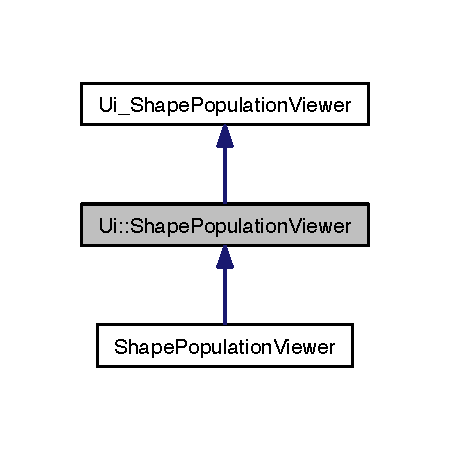
\includegraphics[width=216pt]{class_ui_1_1_shape_population_viewer__inherit__graph}
\end{center}
\end{figure}


Collaboration diagram for Ui\-:\-:Shape\-Population\-Viewer\-:\nopagebreak
\begin{figure}[H]
\begin{center}
\leavevmode
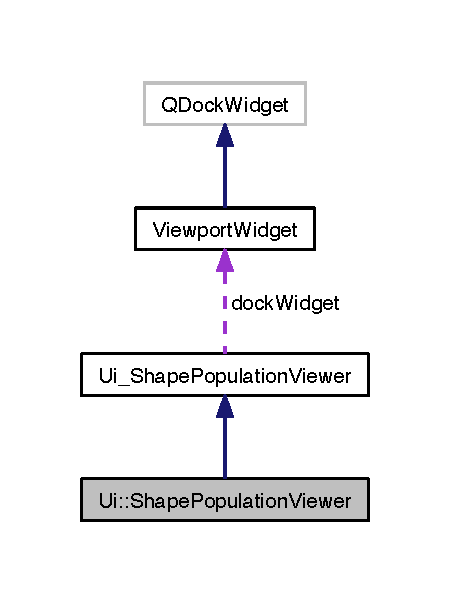
\includegraphics[width=216pt]{class_ui_1_1_shape_population_viewer__coll__graph}
\end{center}
\end{figure}
\subsection*{Additional Inherited Members}


The documentation for this class was generated from the following file\-:\begin{DoxyCompactItemize}
\item 
ui\-\_\-\-Shape\-Population\-Viewer.\-h\end{DoxyCompactItemize}

\hypertarget{class_ui___shape_population_viewer}{\section{Ui\-\_\-\-Shape\-Population\-Viewer Class Reference}
\label{class_ui___shape_population_viewer}\index{Ui\-\_\-\-Shape\-Population\-Viewer@{Ui\-\_\-\-Shape\-Population\-Viewer}}
}


Inheritance diagram for Ui\-\_\-\-Shape\-Population\-Viewer\-:\nopagebreak
\begin{figure}[H]
\begin{center}
\leavevmode
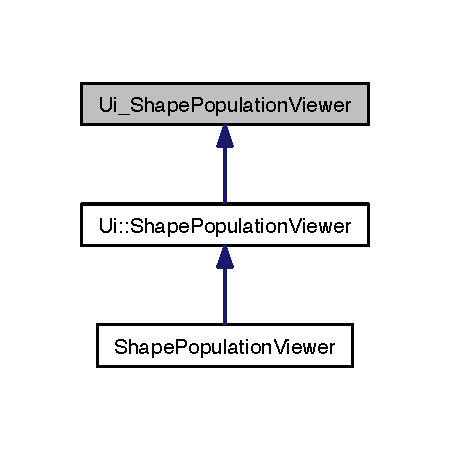
\includegraphics[width=216pt]{class_ui___shape_population_viewer__inherit__graph}
\end{center}
\end{figure}


Collaboration diagram for Ui\-\_\-\-Shape\-Population\-Viewer\-:\nopagebreak
\begin{figure}[H]
\begin{center}
\leavevmode
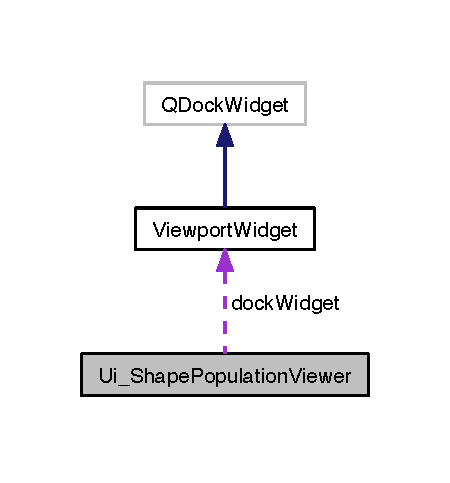
\includegraphics[width=216pt]{class_ui___shape_population_viewer__coll__graph}
\end{center}
\end{figure}
\subsection*{Public Member Functions}
\begin{DoxyCompactItemize}
\item 
\hypertarget{class_ui___shape_population_viewer_a58ba0c071f45f4e2f676d7e47dadbbb3}{void {\bfseries setup\-Ui} (Q\-Main\-Window $\ast$\hyperlink{class_shape_population_viewer}{Shape\-Population\-Viewer})}\label{class_ui___shape_population_viewer_a58ba0c071f45f4e2f676d7e47dadbbb3}

\item 
\hypertarget{class_ui___shape_population_viewer_aebe98684798a7ccdd7d979f3fde23be2}{void {\bfseries retranslate\-Ui} (Q\-Main\-Window $\ast$\hyperlink{class_shape_population_viewer}{Shape\-Population\-Viewer})}\label{class_ui___shape_population_viewer_aebe98684798a7ccdd7d979f3fde23be2}

\end{DoxyCompactItemize}
\subsection*{Public Attributes}
\begin{DoxyCompactItemize}
\item 
\hypertarget{class_ui___shape_population_viewer_a58f4923d6705e47a569ccdaa1ba950ce}{Q\-Action $\ast$ {\bfseries action\-Open\-File}}\label{class_ui___shape_population_viewer_a58f4923d6705e47a569ccdaa1ba950ce}

\item 
\hypertarget{class_ui___shape_population_viewer_ace554b35188e2266e75d55577875b171}{Q\-Action $\ast$ {\bfseries action\-Exit}}\label{class_ui___shape_population_viewer_ace554b35188e2266e75d55577875b171}

\item 
\hypertarget{class_ui___shape_population_viewer_a9ac409dda64e917fe1488ee100820b80}{Q\-Action $\ast$ {\bfseries action\-Print}}\label{class_ui___shape_population_viewer_a9ac409dda64e917fe1488ee100820b80}

\item 
\hypertarget{class_ui___shape_population_viewer_a92290dc77004bc9ef295bce741137e7b}{Q\-Action $\ast$ {\bfseries action\-Help}}\label{class_ui___shape_population_viewer_a92290dc77004bc9ef295bce741137e7b}

\item 
\hypertarget{class_ui___shape_population_viewer_a5528a51653195ff23ff1c8f0b07f3a71}{Q\-Action $\ast$ {\bfseries action\-Save}}\label{class_ui___shape_population_viewer_a5528a51653195ff23ff1c8f0b07f3a71}

\item 
\hypertarget{class_ui___shape_population_viewer_a71a8abf27a03d8433b69f26859b37fbd}{Q\-Action $\ast$ {\bfseries action\-Flip\-\_\-\-Meshes}}\label{class_ui___shape_population_viewer_a71a8abf27a03d8433b69f26859b37fbd}

\item 
\hypertarget{class_ui___shape_population_viewer_ab48a26c5d53762d6669813fe1f6ccfaf}{Q\-Action $\ast$ {\bfseries action\-Write\-\_\-\-Back\-\_\-\-Meshes}}\label{class_ui___shape_population_viewer_ab48a26c5d53762d6669813fe1f6ccfaf}

\item 
\hypertarget{class_ui___shape_population_viewer_a3fed0dc43d988ee2f0a88bd5f41e2f8d}{Q\-Action $\ast$ {\bfseries action\-Open\-\_\-vtk\-\_\-\-Files}}\label{class_ui___shape_population_viewer_a3fed0dc43d988ee2f0a88bd5f41e2f8d}

\item 
\hypertarget{class_ui___shape_population_viewer_aeb8fec16684660d1702cf2d4f1d12f2f}{Q\-Widget $\ast$ {\bfseries centralwidget}}\label{class_ui___shape_population_viewer_aeb8fec16684660d1702cf2d4f1d12f2f}

\item 
\hypertarget{class_ui___shape_population_viewer_af3bc5541822e536de7b4a80d50d90195}{Q\-Grid\-Layout $\ast$ {\bfseries grid\-Layout}}\label{class_ui___shape_population_viewer_af3bc5541822e536de7b4a80d50d90195}

\item 
\hypertarget{class_ui___shape_population_viewer_af5e228584a01908bc1c03518e524637c}{Q\-Group\-Box $\ast$ {\bfseries group\-Box\-\_\-6}}\label{class_ui___shape_population_viewer_af5e228584a01908bc1c03518e524637c}

\item 
\hypertarget{class_ui___shape_population_viewer_ad16b63d2018a2ebb705ff5be049f1f8e}{Q\-Group\-Box $\ast$ {\bfseries group\-Box\-\_\-4}}\label{class_ui___shape_population_viewer_ad16b63d2018a2ebb705ff5be049f1f8e}

\item 
\hypertarget{class_ui___shape_population_viewer_a550f85a97f1beedbb4ed26ff2ad1143b}{Q\-Widget $\ast$ {\bfseries vertical\-Layout\-Widget}}\label{class_ui___shape_population_viewer_a550f85a97f1beedbb4ed26ff2ad1143b}

\item 
\hypertarget{class_ui___shape_population_viewer_a6d6c91184d20792aeb28b7b5044f0abf}{Q\-V\-Box\-Layout $\ast$ {\bfseries vertical\-Layout}}\label{class_ui___shape_population_viewer_a6d6c91184d20792aeb28b7b5044f0abf}

\item 
\hypertarget{class_ui___shape_population_viewer_a64011f16a878e4138f972f03100bd8e5}{Q\-Combo\-Box $\ast$ {\bfseries combo\-Box}}\label{class_ui___shape_population_viewer_a64011f16a878e4138f972f03100bd8e5}

\item 
\hypertarget{class_ui___shape_population_viewer_a645bc1a3805b989bfb60fdd4835c88d6}{Q\-Group\-Box $\ast$ {\bfseries group\-Box\-\_\-5}}\label{class_ui___shape_population_viewer_a645bc1a3805b989bfb60fdd4835c88d6}

\item 
\hypertarget{class_ui___shape_population_viewer_a5ab614d7c8de8e7d5c9f347e6a533776}{Q\-Widget $\ast$ {\bfseries vertical\-Layout\-Widget\-\_\-3}}\label{class_ui___shape_population_viewer_a5ab614d7c8de8e7d5c9f347e6a533776}

\item 
\hypertarget{class_ui___shape_population_viewer_a41bb6c41ce83be21aade5f5f1cc14b4b}{Q\-V\-Box\-Layout $\ast$ {\bfseries vertical\-Layout\-\_\-2}}\label{class_ui___shape_population_viewer_a41bb6c41ce83be21aade5f5f1cc14b4b}

\item 
\hypertarget{class_ui___shape_population_viewer_a1d0b21459e70bf50df0d7b096584baaf}{Q\-Check\-Box $\ast$ {\bfseries check\-Box\-\_\-9}}\label{class_ui___shape_population_viewer_a1d0b21459e70bf50df0d7b096584baaf}

\item 
\hypertarget{class_ui___shape_population_viewer_a9951cfa48bbeac90b3149d41bc5e9b51}{Q\-H\-Box\-Layout $\ast$ {\bfseries horizontal\-Layout\-\_\-7}}\label{class_ui___shape_population_viewer_a9951cfa48bbeac90b3149d41bc5e9b51}

\item 
\hypertarget{class_ui___shape_population_viewer_a9987cfb8cc28c513d88fd4fda358172f}{Q\-Check\-Box $\ast$ {\bfseries check\-Box\-\_\-10}}\label{class_ui___shape_population_viewer_a9987cfb8cc28c513d88fd4fda358172f}

\item 
\hypertarget{class_ui___shape_population_viewer_a76a73443281f9294843ac1e2e67822ce}{Q\-Line\-Edit $\ast$ {\bfseries line\-Edit}}\label{class_ui___shape_population_viewer_a76a73443281f9294843ac1e2e67822ce}

\item 
\hypertarget{class_ui___shape_population_viewer_ab5eb96a308c04fad1070ded37dab571d}{Q\-Label $\ast$ {\bfseries label\-\_\-5}}\label{class_ui___shape_population_viewer_ab5eb96a308c04fad1070ded37dab571d}

\item 
\hypertarget{class_ui___shape_population_viewer_a82b0e1935224c286d02c933847bb539f}{Q\-Check\-Box $\ast$ {\bfseries check\-Box\-\_\-3}}\label{class_ui___shape_population_viewer_a82b0e1935224c286d02c933847bb539f}

\item 
\hypertarget{class_ui___shape_population_viewer_a122d88319567bbd1facdaaca34b2f202}{Q\-Group\-Box $\ast$ {\bfseries group\-Box}}\label{class_ui___shape_population_viewer_a122d88319567bbd1facdaaca34b2f202}

\item 
\hypertarget{class_ui___shape_population_viewer_aa31e5757e3798f9648485c7f48eb3d85}{Q\-Grid\-Layout $\ast$ {\bfseries grid\-Layout\-\_\-3}}\label{class_ui___shape_population_viewer_aa31e5757e3798f9648485c7f48eb3d85}

\item 
\hypertarget{class_ui___shape_population_viewer_a2e81b3943e7cd43edd0bd6d41b42aef7}{Q\-Widget $\ast$ {\bfseries widget}}\label{class_ui___shape_population_viewer_a2e81b3943e7cd43edd0bd6d41b42aef7}

\item 
\hypertarget{class_ui___shape_population_viewer_ae80dc998f4b58c43777c43cf5b2869a0}{Q\-Tool\-Button $\ast$ {\bfseries tool\-Button}}\label{class_ui___shape_population_viewer_ae80dc998f4b58c43777c43cf5b2869a0}

\item 
\hypertarget{class_ui___shape_population_viewer_a933f45c6629c5235a40cb5f5c5baaf88}{Q\-Tool\-Button $\ast$ {\bfseries tool\-Button\-\_\-2}}\label{class_ui___shape_population_viewer_a933f45c6629c5235a40cb5f5c5baaf88}

\item 
\hypertarget{class_ui___shape_population_viewer_aec17295c3295fa64a4c79e60e99b4826}{Q\-Tool\-Button $\ast$ {\bfseries tool\-Button\-\_\-4}}\label{class_ui___shape_population_viewer_aec17295c3295fa64a4c79e60e99b4826}

\item 
\hypertarget{class_ui___shape_population_viewer_a5259557488aa3aaa990b84b9cdab42f4}{Q\-Tool\-Button $\ast$ {\bfseries tool\-Button\-\_\-3}}\label{class_ui___shape_population_viewer_a5259557488aa3aaa990b84b9cdab42f4}

\item 
\hypertarget{class_ui___shape_population_viewer_a83ca98a5531a253095593571c0714d1d}{Q\-Tool\-Button $\ast$ {\bfseries tool\-Button\-\_\-5}}\label{class_ui___shape_population_viewer_a83ca98a5531a253095593571c0714d1d}

\item 
\hypertarget{class_ui___shape_population_viewer_aef925f6808998b14c2f1a1777975a603}{Q\-Tool\-Button $\ast$ {\bfseries tool\-Button\-\_\-6}}\label{class_ui___shape_population_viewer_aef925f6808998b14c2f1a1777975a603}

\item 
\hypertarget{class_ui___shape_population_viewer_a17a3970df680c444831ce36b82e86c30}{\hyperlink{class_viewport_widget}{Viewport\-Widget} $\ast$ {\bfseries dock\-Widget}}\label{class_ui___shape_population_viewer_a17a3970df680c444831ce36b82e86c30}

\item 
\hypertarget{class_ui___shape_population_viewer_a8b9aeca277b4e22cd174bf665d49c6c4}{Q\-Widget $\ast$ {\bfseries dock\-Widget\-Contents}}\label{class_ui___shape_population_viewer_a8b9aeca277b4e22cd174bf665d49c6c4}

\item 
\hypertarget{class_ui___shape_population_viewer_a13b301d656b77abbf223d490f24c05f3}{Q\-Grid\-Layout $\ast$ {\bfseries grid\-Layout\-\_\-2}}\label{class_ui___shape_population_viewer_a13b301d656b77abbf223d490f24c05f3}

\item 
\hypertarget{class_ui___shape_population_viewer_a4321ba9527394aa5dd0ea86904e5c079}{Q\-Scroll\-Area $\ast$ {\bfseries scroll\-Area}}\label{class_ui___shape_population_viewer_a4321ba9527394aa5dd0ea86904e5c079}

\item 
\hypertarget{class_ui___shape_population_viewer_ad4285cc74892781f0419c5efa53a4663}{Q\-Widget $\ast$ {\bfseries scroll\-Area\-Widget\-Contents}}\label{class_ui___shape_population_viewer_ad4285cc74892781f0419c5efa53a4663}

\item 
\hypertarget{class_ui___shape_population_viewer_a23ea5087f7f5c64a93f0f73f0272e143}{Q\-Grid\-Layout $\ast$ {\bfseries grid\-Layout\-\_\-5}}\label{class_ui___shape_population_viewer_a23ea5087f7f5c64a93f0f73f0272e143}

\item 
\hypertarget{class_ui___shape_population_viewer_a62491d50e5e5da4a1253417b27fa9af8}{Q\-Menu\-Bar $\ast$ {\bfseries menu\-Bar}}\label{class_ui___shape_population_viewer_a62491d50e5e5da4a1253417b27fa9af8}

\item 
\hypertarget{class_ui___shape_population_viewer_a643fe8b0da014e88840718671ee9d360}{Q\-Menu $\ast$ {\bfseries menu\-Tools}}\label{class_ui___shape_population_viewer_a643fe8b0da014e88840718671ee9d360}

\item 
\hypertarget{class_ui___shape_population_viewer_a3e1f6eece1982ca2e0ecfea1fe60389e}{Q\-Menu $\ast$ {\bfseries menu\-File}}\label{class_ui___shape_population_viewer_a3e1f6eece1982ca2e0ecfea1fe60389e}

\end{DoxyCompactItemize}


The documentation for this class was generated from the following file\-:\begin{DoxyCompactItemize}
\item 
ui\-\_\-\-Shape\-Population\-Viewer.\-h\end{DoxyCompactItemize}

\hypertarget{class_viewport_widget}{\section{Viewport\-Widget Class Reference}
\label{class_viewport_widget}\index{Viewport\-Widget@{Viewport\-Widget}}
}


Inheritance diagram for Viewport\-Widget\-:


Collaboration diagram for Viewport\-Widget\-:
\subsection*{Public Member Functions}
\begin{DoxyCompactItemize}
\item 
\hypertarget{class_viewport_widget_a0012361ba2ffd4983794291422db7e7a}{{\bfseries Viewport\-Widget} (Q\-Widget $\ast$parent, Q\-Widget $\ast$area\-Conts)}\label{class_viewport_widget_a0012361ba2ffd4983794291422db7e7a}

\item 
\hypertarget{class_viewport_widget_a207a42f641caf95552b0352a458f8447}{Q\-Size {\bfseries size} ()}\label{class_viewport_widget_a207a42f641caf95552b0352a458f8447}

\end{DoxyCompactItemize}
\subsection*{Protected Member Functions}
\begin{DoxyCompactItemize}
\item 
\hypertarget{class_viewport_widget_a319e0b4792e88f86ce11da6ae415930c}{void {\bfseries resize\-Event} (Q\-Resize\-Event $\ast$event)}\label{class_viewport_widget_a319e0b4792e88f86ce11da6ae415930c}

\end{DoxyCompactItemize}


The documentation for this class was generated from the following file\-:\begin{DoxyCompactItemize}
\item 
Viewport\-Widget.\-h\end{DoxyCompactItemize}

\addcontentsline{toc}{part}{Index}
\printindex
\end{document}
